\documentclass[]{article}
\usepackage{lmodern}
\usepackage{amssymb,amsmath}
\usepackage{ifxetex,ifluatex}
\usepackage{fixltx2e} % provides \textsubscript
\ifnum 0\ifxetex 1\fi\ifluatex 1\fi=0 % if pdftex
  \usepackage[T1]{fontenc}
  \usepackage[utf8]{inputenc}
\else % if luatex or xelatex
  \ifxetex
    \usepackage{mathspec}
  \else
    \usepackage{fontspec}
  \fi
  \defaultfontfeatures{Ligatures=TeX,Scale=MatchLowercase}
\fi
% use upquote if available, for straight quotes in verbatim environments
\IfFileExists{upquote.sty}{\usepackage{upquote}}{}
% use microtype if available
\IfFileExists{microtype.sty}{%
\usepackage{microtype}
\UseMicrotypeSet[protrusion]{basicmath} % disable protrusion for tt fonts
}{}
\usepackage[margin=1in]{geometry}
\usepackage{hyperref}
\hypersetup{unicode=true,
            pdftitle={R Independent Study},
            pdfauthor={Enxhi Xhindoli},
            pdfborder={0 0 0},
            breaklinks=true}
\urlstyle{same}  % don't use monospace font for urls
\usepackage{color}
\usepackage{fancyvrb}
\newcommand{\VerbBar}{|}
\newcommand{\VERB}{\Verb[commandchars=\\\{\}]}
\DefineVerbatimEnvironment{Highlighting}{Verbatim}{commandchars=\\\{\}}
% Add ',fontsize=\small' for more characters per line
\usepackage{framed}
\definecolor{shadecolor}{RGB}{248,248,248}
\newenvironment{Shaded}{\begin{snugshade}}{\end{snugshade}}
\newcommand{\KeywordTok}[1]{\textcolor[rgb]{0.13,0.29,0.53}{\textbf{#1}}}
\newcommand{\DataTypeTok}[1]{\textcolor[rgb]{0.13,0.29,0.53}{#1}}
\newcommand{\DecValTok}[1]{\textcolor[rgb]{0.00,0.00,0.81}{#1}}
\newcommand{\BaseNTok}[1]{\textcolor[rgb]{0.00,0.00,0.81}{#1}}
\newcommand{\FloatTok}[1]{\textcolor[rgb]{0.00,0.00,0.81}{#1}}
\newcommand{\ConstantTok}[1]{\textcolor[rgb]{0.00,0.00,0.00}{#1}}
\newcommand{\CharTok}[1]{\textcolor[rgb]{0.31,0.60,0.02}{#1}}
\newcommand{\SpecialCharTok}[1]{\textcolor[rgb]{0.00,0.00,0.00}{#1}}
\newcommand{\StringTok}[1]{\textcolor[rgb]{0.31,0.60,0.02}{#1}}
\newcommand{\VerbatimStringTok}[1]{\textcolor[rgb]{0.31,0.60,0.02}{#1}}
\newcommand{\SpecialStringTok}[1]{\textcolor[rgb]{0.31,0.60,0.02}{#1}}
\newcommand{\ImportTok}[1]{#1}
\newcommand{\CommentTok}[1]{\textcolor[rgb]{0.56,0.35,0.01}{\textit{#1}}}
\newcommand{\DocumentationTok}[1]{\textcolor[rgb]{0.56,0.35,0.01}{\textbf{\textit{#1}}}}
\newcommand{\AnnotationTok}[1]{\textcolor[rgb]{0.56,0.35,0.01}{\textbf{\textit{#1}}}}
\newcommand{\CommentVarTok}[1]{\textcolor[rgb]{0.56,0.35,0.01}{\textbf{\textit{#1}}}}
\newcommand{\OtherTok}[1]{\textcolor[rgb]{0.56,0.35,0.01}{#1}}
\newcommand{\FunctionTok}[1]{\textcolor[rgb]{0.00,0.00,0.00}{#1}}
\newcommand{\VariableTok}[1]{\textcolor[rgb]{0.00,0.00,0.00}{#1}}
\newcommand{\ControlFlowTok}[1]{\textcolor[rgb]{0.13,0.29,0.53}{\textbf{#1}}}
\newcommand{\OperatorTok}[1]{\textcolor[rgb]{0.81,0.36,0.00}{\textbf{#1}}}
\newcommand{\BuiltInTok}[1]{#1}
\newcommand{\ExtensionTok}[1]{#1}
\newcommand{\PreprocessorTok}[1]{\textcolor[rgb]{0.56,0.35,0.01}{\textit{#1}}}
\newcommand{\AttributeTok}[1]{\textcolor[rgb]{0.77,0.63,0.00}{#1}}
\newcommand{\RegionMarkerTok}[1]{#1}
\newcommand{\InformationTok}[1]{\textcolor[rgb]{0.56,0.35,0.01}{\textbf{\textit{#1}}}}
\newcommand{\WarningTok}[1]{\textcolor[rgb]{0.56,0.35,0.01}{\textbf{\textit{#1}}}}
\newcommand{\AlertTok}[1]{\textcolor[rgb]{0.94,0.16,0.16}{#1}}
\newcommand{\ErrorTok}[1]{\textcolor[rgb]{0.64,0.00,0.00}{\textbf{#1}}}
\newcommand{\NormalTok}[1]{#1}
\usepackage{graphicx,grffile}
\makeatletter
\def\maxwidth{\ifdim\Gin@nat@width>\linewidth\linewidth\else\Gin@nat@width\fi}
\def\maxheight{\ifdim\Gin@nat@height>\textheight\textheight\else\Gin@nat@height\fi}
\makeatother
% Scale images if necessary, so that they will not overflow the page
% margins by default, and it is still possible to overwrite the defaults
% using explicit options in \includegraphics[width, height, ...]{}
\setkeys{Gin}{width=\maxwidth,height=\maxheight,keepaspectratio}
\IfFileExists{parskip.sty}{%
\usepackage{parskip}
}{% else
\setlength{\parindent}{0pt}
\setlength{\parskip}{6pt plus 2pt minus 1pt}
}
\setlength{\emergencystretch}{3em}  % prevent overfull lines
\providecommand{\tightlist}{%
  \setlength{\itemsep}{0pt}\setlength{\parskip}{0pt}}
\setcounter{secnumdepth}{0}
% Redefines (sub)paragraphs to behave more like sections
\ifx\paragraph\undefined\else
\let\oldparagraph\paragraph
\renewcommand{\paragraph}[1]{\oldparagraph{#1}\mbox{}}
\fi
\ifx\subparagraph\undefined\else
\let\oldsubparagraph\subparagraph
\renewcommand{\subparagraph}[1]{\oldsubparagraph{#1}\mbox{}}
\fi

%%% Use protect on footnotes to avoid problems with footnotes in titles
\let\rmarkdownfootnote\footnote%
\def\footnote{\protect\rmarkdownfootnote}

%%% Change title format to be more compact
\usepackage{titling}

% Create subtitle command for use in maketitle
\newcommand{\subtitle}[1]{
  \posttitle{
    \begin{center}\large#1\end{center}
    }
}

\setlength{\droptitle}{-2em}

  \title{R Independent Study}
    \pretitle{\vspace{\droptitle}\centering\huge}
  \posttitle{\par}
    \author{Enxhi Xhindoli}
    \preauthor{\centering\large\emph}
  \postauthor{\par}
      \predate{\centering\large\emph}
  \postdate{\par}
    \date{04/29/2019}


\begin{document}
\maketitle

In this report, a logistic regression was constructed in order to obtain
the likelihood of an account churning based off variables utilized
within the model. The logistic regression allows to assess the churn
likelihood of pre-existing accounts.

\subsection{Data Collection}\label{data-collection}

The telecomunication company provided the LSU team with different
datasets about demographics and rate changes. For the scope of this
project, only a subset of the whole dataset was used. The variable
BAN\_SEQ is the ID which identifies a unique customer.

\begin{Shaded}
\begin{Highlighting}[]
\NormalTok{RCU <-}\StringTok{ }\KeywordTok{read.csv}\NormalTok{(}\KeywordTok{here}\NormalTok{(}\StringTok{'Data'}\NormalTok{, }\StringTok{'RateChangeUnique.csv'}\NormalTok{),}\DataTypeTok{sep =}\StringTok{","}\NormalTok{, }\DataTypeTok{header =} \OtherTok{TRUE}\NormalTok{)}
\NormalTok{DEMO <-}\StringTok{ }\KeywordTok{read.csv}\NormalTok{(}\KeywordTok{here}\NormalTok{(}\StringTok{'Data'}\NormalTok{, }\StringTok{'DEMO.csv'}\NormalTok{), }\DataTypeTok{sep =}\StringTok{","}\NormalTok{, }\DataTypeTok{header=}\OtherTok{TRUE}\NormalTok{)}
\NormalTok{DF <-}\StringTok{ }\KeywordTok{full_join}\NormalTok{(DEMO,RCU, }\DataTypeTok{by =} \StringTok{"BAN_SEQ"}\NormalTok{)}
\end{Highlighting}
\end{Shaded}

\subsubsection{Scraping}\label{scraping}

In order to add some information about the income, a table containing
the average income per state was brought from the website into the
Global Environment of Rstudio.

\begin{Shaded}
\begin{Highlighting}[]
\NormalTok{income <-}\StringTok{ }\KeywordTok{read_html}\NormalTok{(}\StringTok{"https://www.infoplease.com/business-finance/poverty-and-income/capita-personal-income-state"}\NormalTok{)}\OperatorTok
\StringTok{  }\KeywordTok{html_node}\NormalTok{(}\DataTypeTok{css =} \StringTok{"#A0104653"}\NormalTok{)}\OperatorTok
\StringTok{  }\KeywordTok{html_table}\NormalTok{()}
\end{Highlighting}
\end{Shaded}

For the purpose of this project, only the column showing the average
income of each state in 2015 was kept.

\begin{Shaded}
\begin{Highlighting}[]
\NormalTok{income <-}\StringTok{ }\KeywordTok{as_tibble}\NormalTok{(income)}
\NormalTok{income <-}\StringTok{ }\KeywordTok{select}\NormalTok{(income, State,}\StringTok{`}\DataTypeTok{2015}\StringTok{`}\NormalTok{)}
\NormalTok{income[}\DecValTok{1}\OperatorTok{:}\DecValTok{3}\NormalTok{,]}
\end{Highlighting}
\end{Shaded}

\begin{verbatim}
## # A tibble: 3 x 2
##   State   `2015` 
##   <chr>   <chr>  
## 1 Alabama $38,965
## 2 Alaska  55,940 
## 3 Arizona 39,060
\end{verbatim}

To change the format of the values in this column, as they need to be
homogeneous, stringr package was used.

\begin{Shaded}
\begin{Highlighting}[]
\NormalTok{income <-}\StringTok{ }\NormalTok{income }\OperatorTok
\StringTok{  }\KeywordTok{mutate}\NormalTok{(}\StringTok{`}\DataTypeTok{2015}\StringTok{`}\NormalTok{=}\KeywordTok{str_extract_all}\NormalTok{(}\StringTok{`}\DataTypeTok{2015}\StringTok{`}\NormalTok{,}\StringTok{"[0-9]+"}\NormalTok{))}\OperatorTok
\StringTok{  }\KeywordTok{mutate}\NormalTok{(}\StringTok{`}\DataTypeTok{2015}\StringTok{`}\NormalTok{=}\KeywordTok{map_chr}\NormalTok{(}\StringTok{`}\DataTypeTok{2015}\StringTok{`}\NormalTok{,paste,}\DataTypeTok{collapse=}\StringTok{""}\NormalTok{))}

\NormalTok{income <-}\StringTok{ }\KeywordTok{as.data.frame}\NormalTok{(income)}
\KeywordTok{names}\NormalTok{(income)[}\KeywordTok{names}\NormalTok{(income) }\OperatorTok{==}\StringTok{ "2015"}\NormalTok{] <-}\StringTok{ "AVG_INCOME_2015"}
\KeywordTok{names}\NormalTok{(income)[}\KeywordTok{names}\NormalTok{(income) }\OperatorTok{==}\StringTok{ "State"}\NormalTok{] <-}\StringTok{ "STATE"}
\end{Highlighting}
\end{Shaded}

In the dataset provided by the company, the states are represented only
with their abbreviation. Therefore, another table, - containing the
states and their abbreviations,- was extracted from the following
website. The table included also the Commonwealth territories which were
dropped from the dataset.

\begin{Shaded}
\begin{Highlighting}[]
\NormalTok{states <-}\StringTok{ }\KeywordTok{read_html}\NormalTok{(}\StringTok{"https://www.50states.com/abbreviations.htm"}\NormalTok{) }\OperatorTok
\StringTok{  }\KeywordTok{html_node}\NormalTok{(}\StringTok{"[class='spaced stripedRows']"}\NormalTok{)}\OperatorTok
\StringTok{  }\KeywordTok{html_table}\NormalTok{()}

\NormalTok{states <-}\StringTok{ }\KeywordTok{as.data.frame}\NormalTok{(states)}
\NormalTok{states <-}\StringTok{ }\NormalTok{states[}\OperatorTok{-}\NormalTok{(}\DecValTok{51}\OperatorTok{:}\DecValTok{67}\NormalTok{),]}

\KeywordTok{names}\NormalTok{(states)[}\KeywordTok{names}\NormalTok{(states) }\OperatorTok{==}\StringTok{ "US State:"}\NormalTok{] <-}\StringTok{ "STATE"}
\KeywordTok{names}\NormalTok{(states)[}\KeywordTok{names}\NormalTok{(states) }\OperatorTok{==}\StringTok{ "Abbreviation:"}\NormalTok{] <-}\StringTok{ "STATE_ABBREVIATION"}
\KeywordTok{colnames}\NormalTok{(states)}
\end{Highlighting}
\end{Shaded}

\begin{verbatim}
## [1] "STATE"              "STATE_ABBREVIATION"
\end{verbatim}

At this point, the two tables were merged by the column ``STATE''.

\begin{Shaded}
\begin{Highlighting}[]
\NormalTok{Income_per_state <-}\StringTok{ }\KeywordTok{merge}\NormalTok{(states,income,}\DataTypeTok{by=}\StringTok{"STATE"}\NormalTok{)}
\KeywordTok{head}\NormalTok{(Income_per_state)}
\end{Highlighting}
\end{Shaded}

\begin{verbatim}
##        STATE STATE_ABBREVIATION AVG_INCOME_2015
## 1    Alabama                 AL           38965
## 2     Alaska                 AK           55940
## 3    Arizona                 AZ           39060
## 4   Arkansas                 AR           39107
## 5 California                 CA           52651
## 6   Colorado                 CO           50410
\end{verbatim}

Finally, to create the final dataset, this table was merged with the csv
dataset provided by the company.

\begin{Shaded}
\begin{Highlighting}[]
\KeywordTok{names}\NormalTok{(DF)[}\KeywordTok{names}\NormalTok{(DF) }\OperatorTok{==}\StringTok{ "STATE"}\NormalTok{] <-}\StringTok{ "STATE_ABBREVIATION"}
\NormalTok{DF1 <-}\StringTok{ }\KeywordTok{left_join}\NormalTok{(DF,Income_per_state, }\DataTypeTok{by =} \StringTok{"STATE_ABBREVIATION"}\NormalTok{)}
\end{Highlighting}
\end{Shaded}

\subsection{Data preparation}\label{data-preparation}

For the purpose of this analysis, only the subset of the observations
belonging to the year 2015 will be considered. Because R recognizes
SNAPSHOT\_DATE as a factor,first it needs to be converted to a
character, and then to a date.

\begin{Shaded}
\begin{Highlighting}[]
\NormalTok{DF1}\OperatorTok{$}\NormalTok{SNAPSHOT_DATE <-}\StringTok{ }\KeywordTok{as.character}\NormalTok{(DF1}\OperatorTok{$}\NormalTok{SNAPSHOT_DATE)}
\NormalTok{DF1}\OperatorTok{$}\NormalTok{SNAPSHOT_DATE <-}\StringTok{ }\KeywordTok{as.Date}\NormalTok{(DF1}\OperatorTok{$}\NormalTok{SNAPSHOT_DATE, }\DataTypeTok{format =} \StringTok{"%m/%d/%Y"}\NormalTok{)}
\end{Highlighting}
\end{Shaded}

\begin{Shaded}
\begin{Highlighting}[]
\NormalTok{DF2 <-DF1 }\OperatorTok\StringTok{ }
\StringTok{  }\KeywordTok{filter}\NormalTok{(SNAPSHOT_DATE}\OperatorTok{>}\StringTok{'2014-12-31'} \OperatorTok{&}\StringTok{ }\NormalTok{SNAPSHOT_DATE}\OperatorTok{<}\StringTok{'2016-01-31'}\NormalTok{)}

\KeywordTok{length}\NormalTok{(}\KeywordTok{unique}\NormalTok{(DF2}\OperatorTok{$}\NormalTok{SNAPSHOT_DATE))}
\end{Highlighting}
\end{Shaded}

\begin{verbatim}
## [1] 12
\end{verbatim}

\begin{Shaded}
\begin{Highlighting}[]
\KeywordTok{unique}\NormalTok{(DF2}\OperatorTok{$}\NormalTok{SNAPSHOT_DATE)}
\end{Highlighting}
\end{Shaded}

\begin{verbatim}
##  [1] "2015-04-30" "2015-01-31" "2015-07-31" "2015-06-30" "2015-05-31"
##  [6] "2015-10-31" "2015-12-31" "2015-03-31" "2015-02-28" "2015-08-31"
## [11] "2015-09-30" "2015-11-30"
\end{verbatim}

From the dataset, it can be clearly seen that the variable
CVGENDERCODE1, which is showing the gender, has more than two
occurrences. For practical reasons, the name of the column was first
changed, and some inspections about it were made.

\begin{Shaded}
\begin{Highlighting}[]
\KeywordTok{names}\NormalTok{(DF2)[}\KeywordTok{names}\NormalTok{(DF2) }\OperatorTok{==}\StringTok{ "CVGENDERCODE1"}\NormalTok{] <-}\StringTok{ "GENDER"}
\NormalTok{DF2}\OperatorTok{$}\NormalTok{GENDER <-}\StringTok{ }\KeywordTok{as.character}\NormalTok{(DF2}\OperatorTok{$}\NormalTok{GENDER)}
\KeywordTok{unique}\NormalTok{(DF2}\OperatorTok{$}\NormalTok{GENDER)}
\end{Highlighting}
\end{Shaded}

\begin{verbatim}
## [1] "M"    "U"    "F"    "null" NA
\end{verbatim}

The observations containing values such as: U and null were converted to
NA. In this dataset, 22\% of the obseravtions have missing values for
gender.

\begin{Shaded}
\begin{Highlighting}[]
\NormalTok{DF2}\OperatorTok{$}\NormalTok{GENDER <-}\StringTok{ }\KeywordTok{revalue}\NormalTok{(DF2}\OperatorTok{$}\NormalTok{GENDER, }\KeywordTok{c}\NormalTok{(}\StringTok{"U"}\NormalTok{=}\OtherTok{NA}\NormalTok{))}
\NormalTok{DF2}\OperatorTok{$}\NormalTok{GENDER <-}\StringTok{ }\KeywordTok{revalue}\NormalTok{(DF2}\OperatorTok{$}\NormalTok{GENDER, }\KeywordTok{c}\NormalTok{(}\StringTok{"null"}\NormalTok{=}\OtherTok{NA}\NormalTok{))}
\KeywordTok{count}\NormalTok{(DF2}\OperatorTok{$}\NormalTok{GENDER}\OperatorTok{==}\StringTok{'NA'}\NormalTok{)}
\end{Highlighting}
\end{Shaded}

Inspections were made also for the variable EDUCATIONAL\_LEVEL.

\begin{Shaded}
\begin{Highlighting}[]
\KeywordTok{unique}\NormalTok{(DF2}\OperatorTok{$}\NormalTok{EDUCATION_LEVEL)}
\end{Highlighting}
\end{Shaded}

\begin{verbatim}
## [1] 5    2    4    7    #N/D 1    3    6    <NA>
## Levels: #N/D 1 2 3 4 5 6 7
\end{verbatim}

\begin{Shaded}
\begin{Highlighting}[]
\NormalTok{DF2}\OperatorTok{$}\NormalTok{EDUCATION_LEVEL <-}\StringTok{ }\KeywordTok{revalue}\NormalTok{(DF2}\OperatorTok{$}\NormalTok{EDUCATION_LEVEL, }\KeywordTok{c}\NormalTok{(}\StringTok{"#N/D"}\NormalTok{=}\OtherTok{NA}\NormalTok{))}
\end{Highlighting}
\end{Shaded}

To see how the customer's paying rate has changed a new variable was
created as difference between CURR\_PAYING\_RATE and
PRIOR\_PAYING\_RATE.

Given the definition of customer churn as \emph{``Customers who stopped
using company's product or service during a certain time frame''}, for
the creation of variable ``CHURN'' the CURR\_QTY and PRIOR\_QTY were
taken into consideration. The two variables refer respectively to the
current and prior quantity of products purchased by the single customer.

\begin{Shaded}
\begin{Highlighting}[]
\NormalTok{DF3}\OperatorTok{$}\NormalTok{CHURN <-}\StringTok{ }\KeywordTok{ifelse}\NormalTok{(DF3}\OperatorTok{$}\NormalTok{CURR_QTY }\OperatorTok{>=}\StringTok{ }\NormalTok{DF3}\OperatorTok{$}\NormalTok{PRIOR_QTY,}\DecValTok{0}\NormalTok{,}\DecValTok{1}\NormalTok{)}
\end{Highlighting}
\end{Shaded}

To make this analysis even more dynamic, the binary variable NEW\_CUST
was created. As the name reveals, it shows whether a person is a new
customer in 2015 or not.

\begin{Shaded}
\begin{Highlighting}[]
\NormalTok{DF3}\OperatorTok{$}\NormalTok{NEW_CUST <-}\StringTok{ }\KeywordTok{if_else}\NormalTok{(DF3}\OperatorTok{$}\NormalTok{CURR_QTY }\OperatorTok{>}\StringTok{ }\DecValTok{0} \OperatorTok{&}\StringTok{ }\NormalTok{DF3}\OperatorTok{$}\NormalTok{PRIOR_QTY }\OperatorTok{==}\StringTok{ }\DecValTok{0}\NormalTok{,}\DecValTok{1}\NormalTok{,}\DecValTok{0}\NormalTok{)}
\NormalTok{DF3}\OperatorTok{$}\NormalTok{NEW_CUST <-}\StringTok{ }\KeywordTok{factor}\NormalTok{(DF3}\OperatorTok{$}\NormalTok{NEW_CUST)}
\end{Highlighting}
\end{Shaded}

\subsection{Visualization}\label{visualization}

The first graph shows how the number of customers has changed during the
year and how many new customers there are each month.

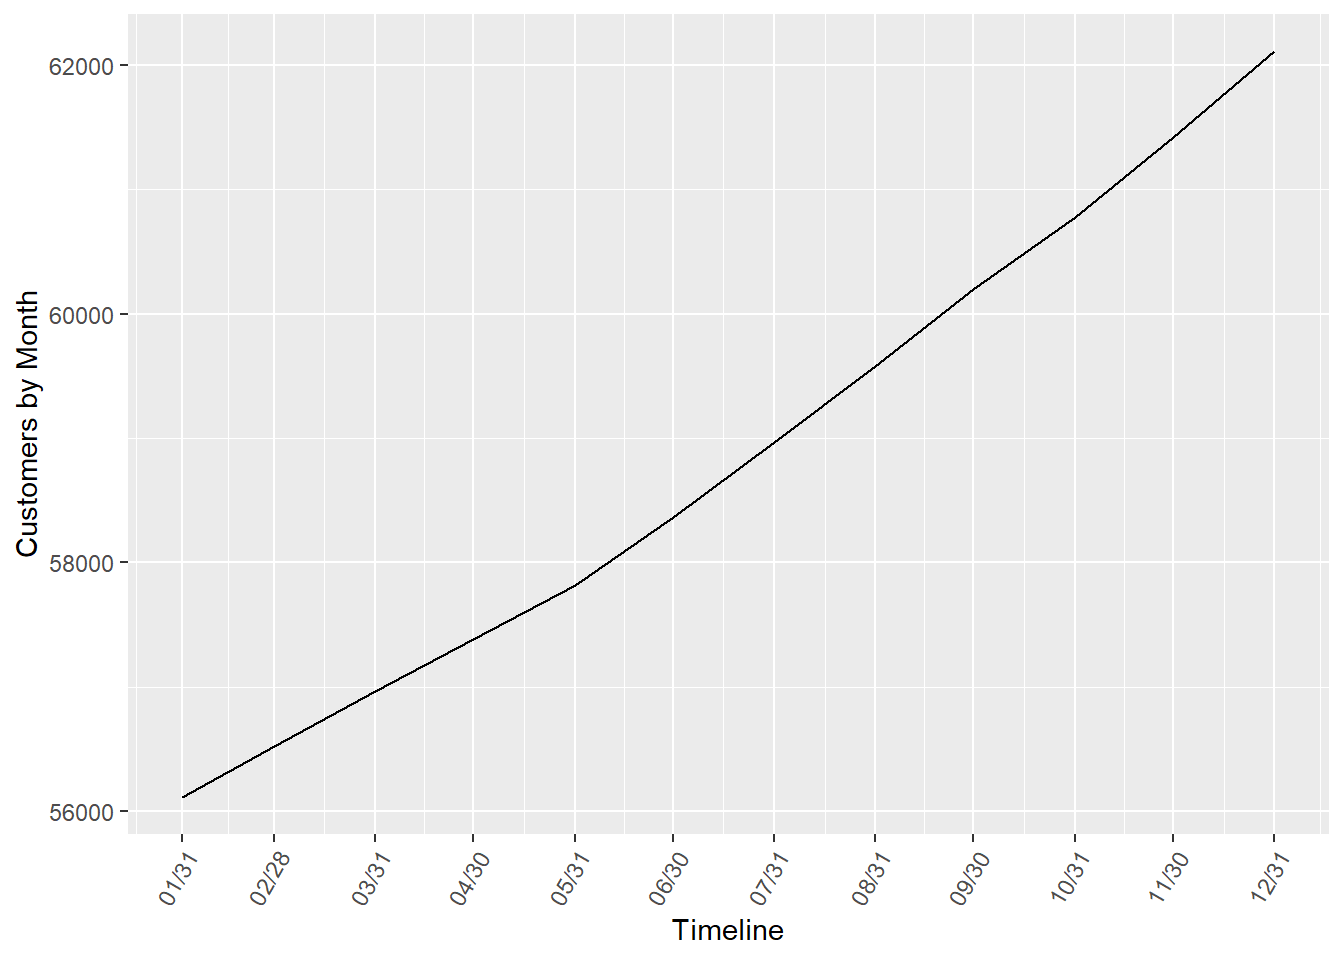
\includegraphics{Project_files/figure-latex/unnamed-chunk-23-1.pdf}

To see the count of customers in each state, a barchart was used.

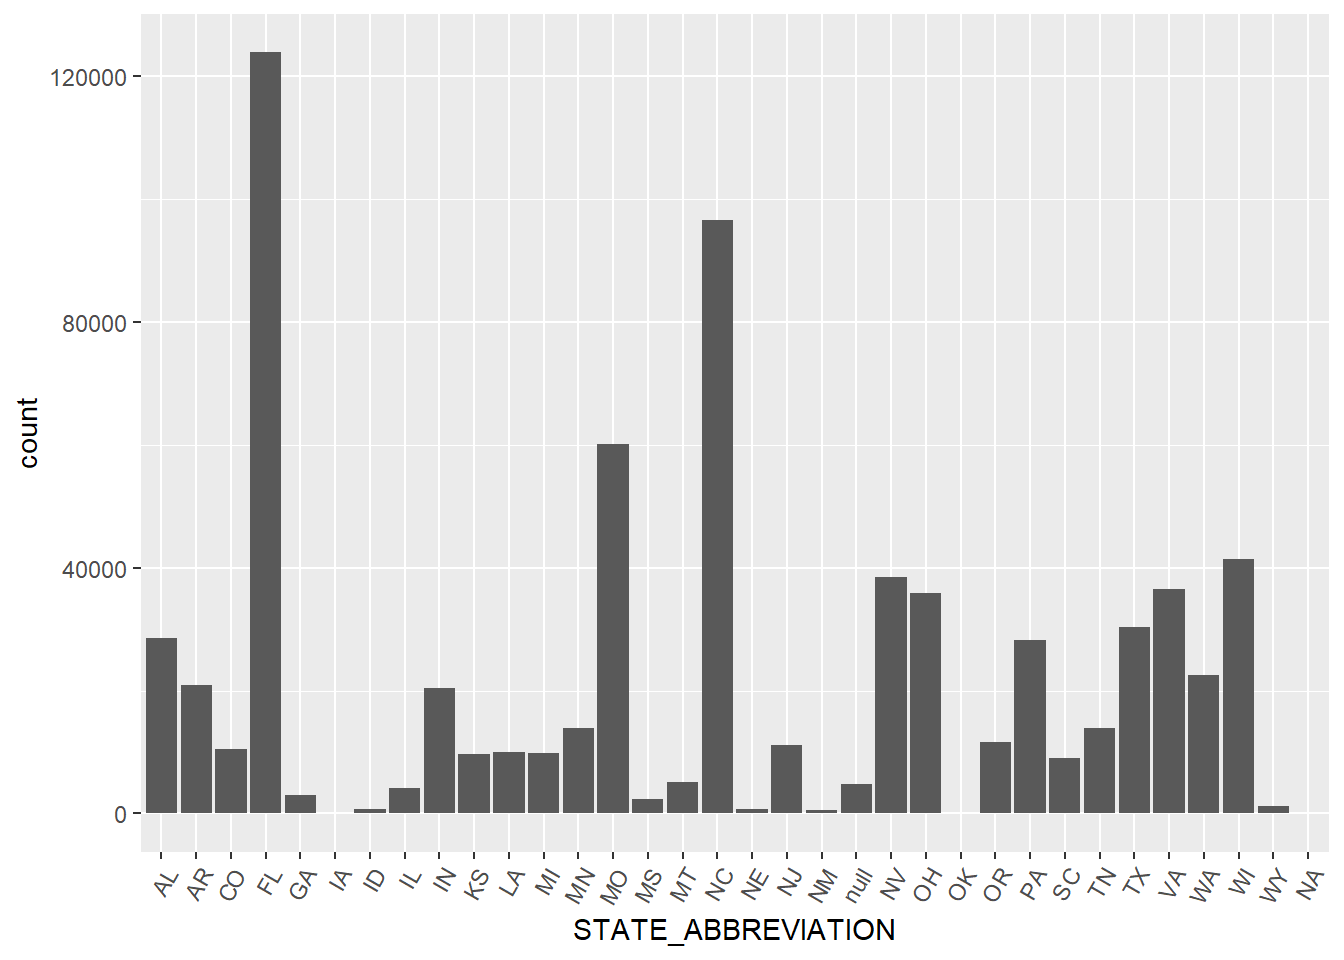
\includegraphics{Project_files/figure-latex/unnamed-chunk-24-1.pdf}

Now that it is known how many customers there are in each state, it
could be interesting to figure out how many of those customers are male
and female.

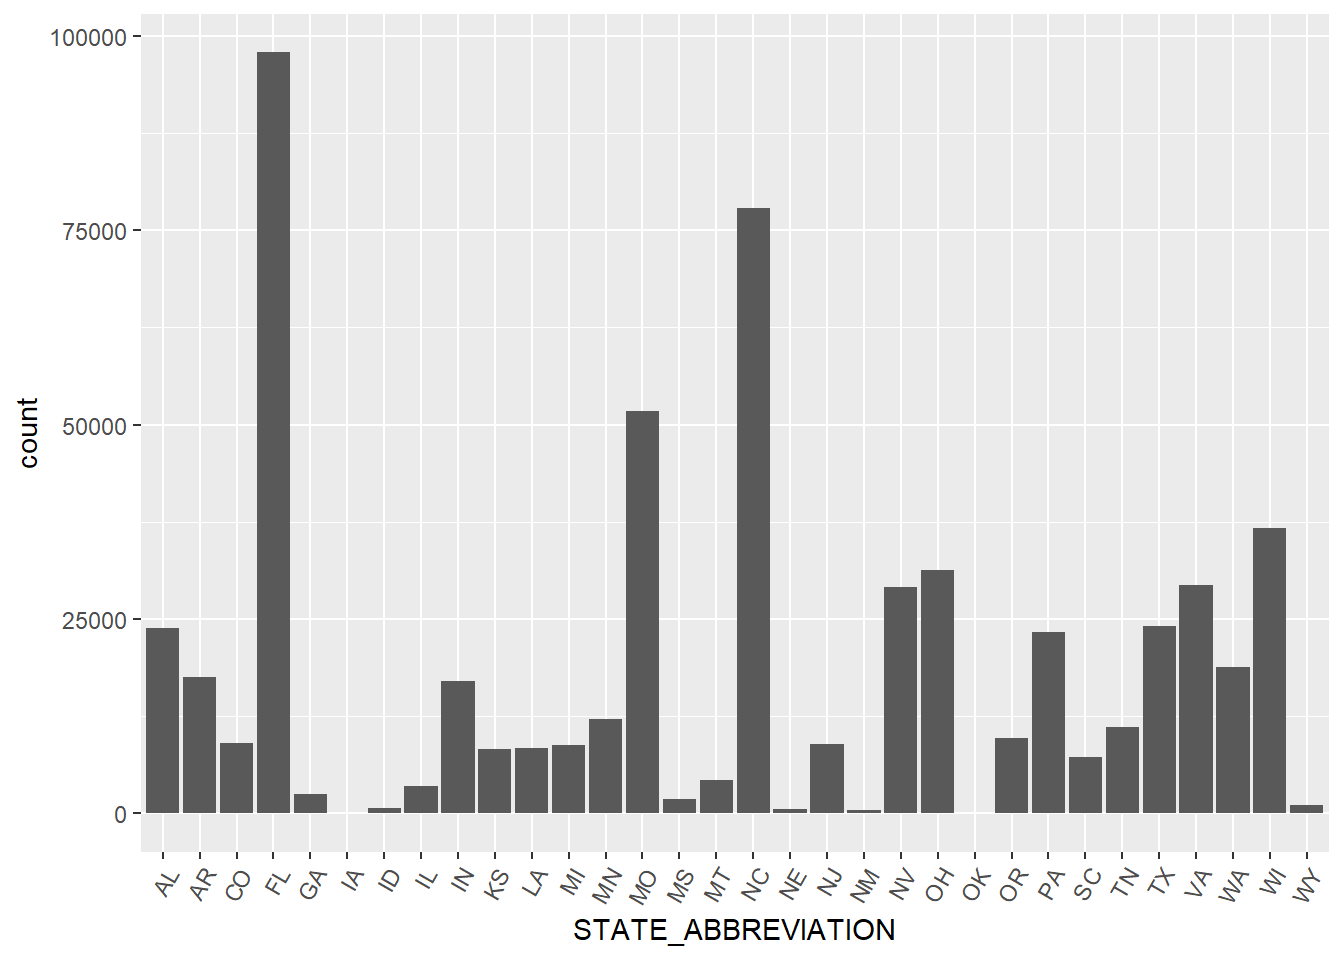
\includegraphics{Project_files/figure-latex/unnamed-chunk-25-1.pdf}

Furthermore, we want se see the correlation between the change in paying
rate and the number of calls.

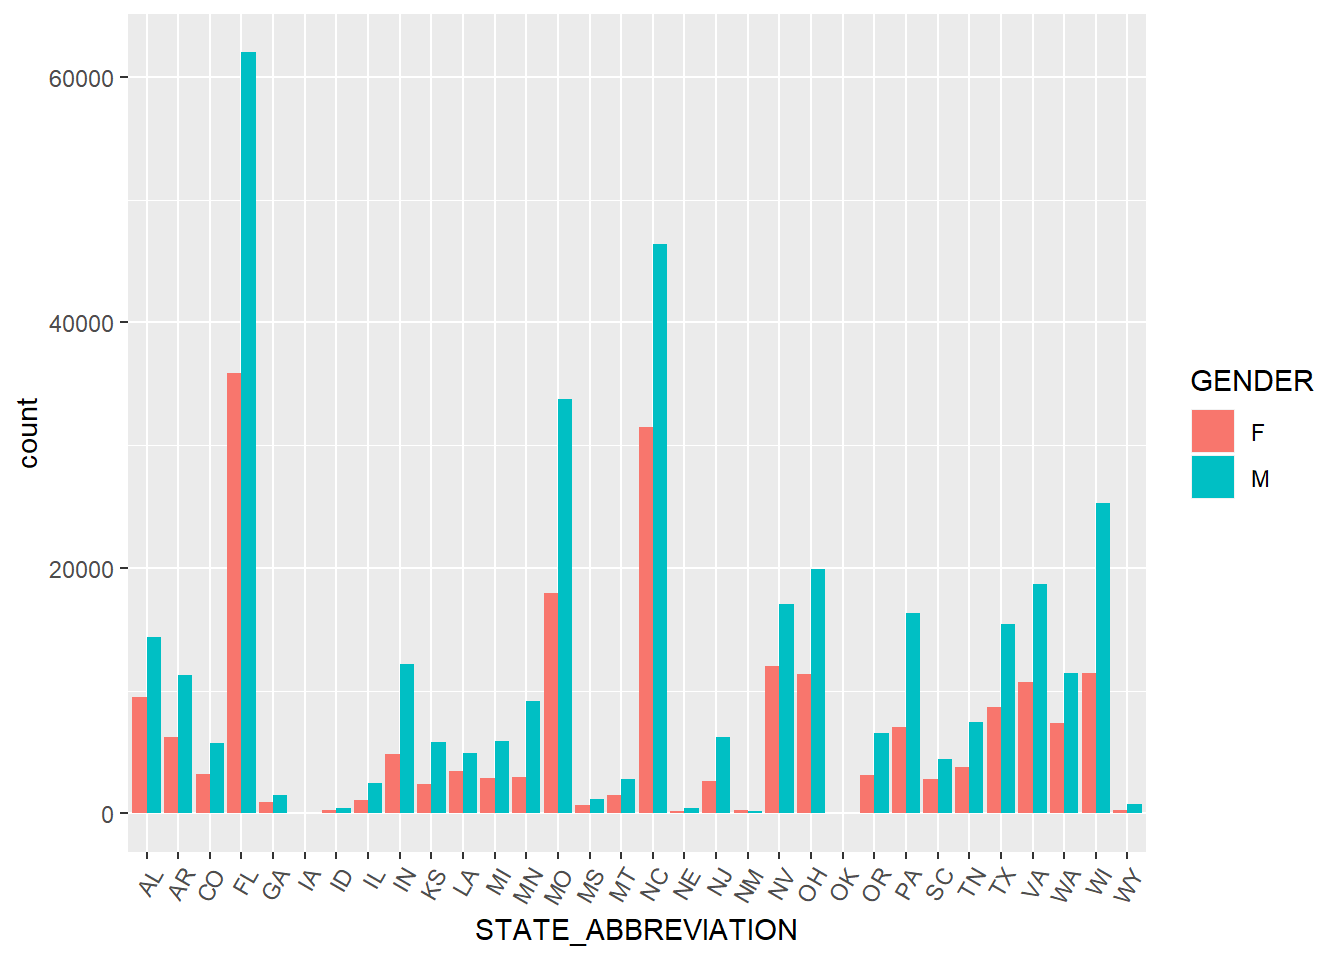
\includegraphics{Project_files/figure-latex/unnamed-chunk-26-1.pdf}

\subsection{Builging a Logistic Regression model to predict
CHURN}\label{builging-a-logistic-regression-model-to-predict-churn}

The objective of the Churn predictive model is to assign to the
customers a measure of the propensity to abandonment (called score).
However, before building a model, it is necessary to see how many
instances of CHURN there are in the dataset.

\begin{Shaded}
\begin{Highlighting}[]
\KeywordTok{table}\NormalTok{(DF3}\OperatorTok{$}\NormalTok{CHURN)}
\end{Highlighting}
\end{Shaded}

\begin{verbatim}
## 
##      0      1 
## 697007   9204
\end{verbatim}

Since the event of churn is a rare event, to maximize the possibility of
developing a model on a sample basis extensible in a robust way also on
the total population, all the cases of abandonment detected in the
analysis period were considered within the sample, while the cases of
``no churn'' were narrowed down (undersampling). The sample was
therefore constructed as follows: 25\% formed by units presenting the
``abandonment'' event (made up of all the customers lost during the
analysis period) and 75\% formed by units that do not have the
``abandonment'' event ( randomly extracted from all customers who have
not left).

\begin{Shaded}
\begin{Highlighting}[]
\NormalTok{DF4 <-}\StringTok{ }\KeywordTok{na.omit}\NormalTok{(DF3)}
\CommentTok{# Split the data into training and test set}
\KeywordTok{set.seed}\NormalTok{(}\DecValTok{123}\NormalTok{)}
\NormalTok{training.samples <-}\StringTok{ }\NormalTok{DF4}\OperatorTok{$}\NormalTok{CHURN }\OperatorTok\StringTok{ }
\StringTok{  }\KeywordTok{createDataPartition}\NormalTok{(}\DataTypeTok{p =} \FloatTok{0.7}\NormalTok{, }\DataTypeTok{list =} \OtherTok{FALSE}\NormalTok{)}
\NormalTok{train.data  <-}\StringTok{ }\NormalTok{DF4[training.samples, ]}
\NormalTok{test.data <-}\StringTok{ }\NormalTok{DF4[}\OperatorTok{-}\NormalTok{training.samples, ]}
\CommentTok{# imbalance on training set}
\KeywordTok{table}\NormalTok{(train.data}\OperatorTok{$}\NormalTok{CHURN)}
\end{Highlighting}
\end{Shaded}

\begin{verbatim}
## 
##      0      1 
## 398775   5334
\end{verbatim}

\begin{Shaded}
\begin{Highlighting}[]
\CommentTok{# balanced data set with under-sampling}
\NormalTok{data.balanced.under <-}\StringTok{ }\KeywordTok{ovun.sample}\NormalTok{(CHURN}\OperatorTok{~}\NormalTok{CREDIT_CLASS}\OperatorTok{+}\NormalTok{NEW_CUST}\OperatorTok{+}\NormalTok{CALL_COUNT}\OperatorTok{+}\NormalTok{AGE}\OperatorTok{+}\NormalTok{GENDER}\OperatorTok{+}\NormalTok{EDUCATION_LEVEL}\OperatorTok{+}\NormalTok{AVG_INCOME_}\DecValTok{2015}\NormalTok{, }\DataTypeTok{data=}\NormalTok{train.data, }\DataTypeTok{p=}\FloatTok{0.25}\NormalTok{, }\DataTypeTok{seed=}\DecValTok{1}\NormalTok{, }\DataTypeTok{method=}\StringTok{"under"}\NormalTok{)}\OperatorTok{$}\NormalTok{data}
\KeywordTok{table}\NormalTok{(data.balanced.under}\OperatorTok{$}\NormalTok{CHURN)}
\end{Highlighting}
\end{Shaded}

\begin{verbatim}
## 
##     0     1 
## 15964  5334
\end{verbatim}

Now a logistic regression model is created based on training balanced
data.

\begin{verbatim}
## 
## Call:
## glm(formula = CHURN ~ CREDIT_CLASS + NEW_CUST + CALL_COUNT + 
##     GENDER + EDUCATION_LEVEL + AVG_INCOME_2015, family = binomial, 
##     data = data.balanced.under)
## 
## Deviance Residuals: 
##     Min       1Q   Median       3Q      Max  
## -3.5356  -0.7453  -0.6597   0.3385   1.8933  
## 
## Coefficients:
##                    Estimate Std. Error z value Pr(>|z|)    
## (Intercept)      -1.633e+00  2.294e-01  -7.120 1.08e-12 ***
## CREDIT_CLASS2     4.022e-01  8.804e-02   4.568 4.92e-06 ***
## CREDIT_CLASS3     3.302e-01  7.808e-02   4.229 2.35e-05 ***
## CREDIT_CLASS4     3.197e-01  9.267e-02   3.449 0.000562 ***
## CREDIT_CLASS5     7.324e-01  2.133e-01   3.434 0.000596 ***
## CREDIT_CLASS6     1.467e-01  7.262e-02   2.020 0.043384 *  
## CREDIT_CLASS7    -1.502e+01  2.400e+03  -0.006 0.995005    
## CREDIT_CLASS8     1.205e+00  2.154e-01   5.594 2.22e-08 ***
## CREDIT_CLASS9     1.994e-02  2.549e-01   0.078 0.937660    
## CREDIT_CLASSA    -7.103e-01  5.062e-01  -1.403 0.160522    
## CREDIT_CLASSH     1.953e-01  1.160e+00   0.168 0.866321    
## CREDIT_CLASSP     1.677e+01  2.400e+03   0.007 0.994423    
## CREDIT_CLASSU    -1.502e+01  1.200e+03  -0.013 0.990008    
## CREDIT_CLASSZ     1.156e+00  1.420e+00   0.814 0.415403    
## NEW_CUST1        -2.073e+01  1.184e+02  -0.175 0.860977    
## CALL_COUNT        3.937e-02  1.488e-03  26.467  < 2e-16 ***
## GENDERM          -2.439e-02  3.394e-02  -0.719 0.472391    
## EDUCATION_LEVEL2  1.662e-01  1.396e-01   1.191 0.233782    
## EDUCATION_LEVEL3  7.239e-02  5.338e-01   0.136 0.892122    
## EDUCATION_LEVEL4  1.319e-01  1.362e-01   0.969 0.332723    
## EDUCATION_LEVEL5  6.286e-02  1.311e-01   0.480 0.631566    
## EDUCATION_LEVEL6  1.264e-01  2.269e-01   0.557 0.577352    
## EDUCATION_LEVEL7  2.294e-01  2.030e-01   1.130 0.258475    
## AVG_INCOME_2015  -3.208e-07  4.059e-06  -0.079 0.936997    
## ---
## Signif. codes:  0 '***' 0.001 '**' 0.01 '*' 0.05 '.' 0.1 ' ' 1
## 
## (Dispersion parameter for binomial family taken to be 1)
## 
##     Null deviance: 23974  on 21297  degrees of freedom
## Residual deviance: 22756  on 21274  degrees of freedom
## AIC: 22804
## 
## Number of Fisher Scoring iterations: 15
\end{verbatim}

The model was then applied to the test data.

\begin{verbatim}
## 
## Call: 
## accuracy.meas(response = test.data$CHURN, predicted = probabilities)
## 
## Examples are labelled as positive when predicted is greater than 0.5 
## 
## precision: 0.034
## recall: 0.056
## F: 0.021
\end{verbatim}


\end{document}
